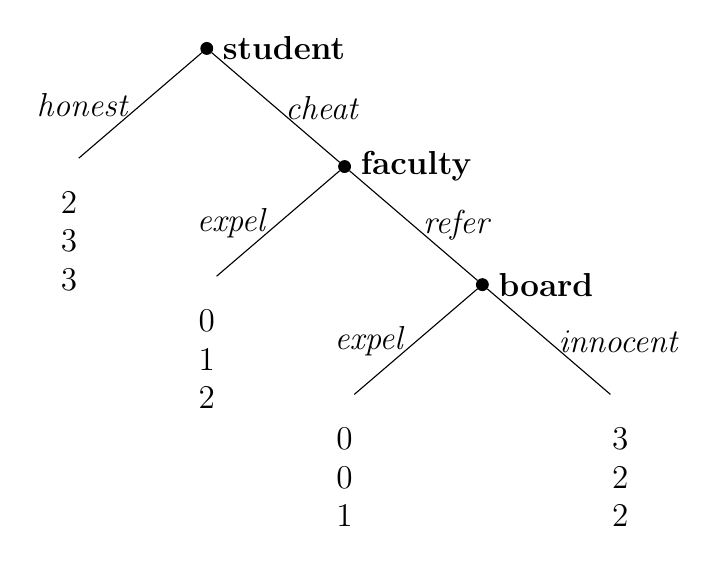
\begin{tikzpicture}[scale=1.0,font=\large]
\tikzstyle{solid node}=[circle,draw,inner sep=1.5,fill=black]
\tikzstyle{level 1}=[level distance=15mm,sibling distance=3.5cm]
\tikzstyle{level 2}=[level distance=15mm,sibling distance=3.5cm]
\tikzstyle{level 3}=[level distance=15mm,sibling distance=3.5cm]

\node(0)[solid node,label=right:{\textbf{student}}]{}
    child{node[label=below:{
            \begin{tabular}{c}
                 {2} \\
                 {3} \\
                 {3} \\
            \end{tabular}
        }]{} 
    edge from parent node[left]{\textit{honest}}}
    child{node[solid node,label=right:{\textbf{faculty}}]{} 
        child{node(1)[label=below:{
            \begin{tabular}{c}
                 {0}  \\
                 {1} \\
                 {2} \\
            \end{tabular}
        }]{} 
        edge from parent node[left]{\textit{expel}} 
        }
        child{node(2)[solid node, label=right:{\textbf{board}}]{} 
            child{node[label=below:{
                \begin{tabular}{c}
                    {0} \\
                    {0} \\
                    {1} \\
                \end{tabular}
                }]{} 
            edge from parent node[left]{\textit{expel}} 
            }
            child{node[label=below:{
                \begin{tabular}{c}
                     {3} \\
                     {2} \\
                     {2} \\
                \end{tabular}
            }]{} 
            edge from parent node[right]{\textit{innocent}} 
            }
        edge from parent node[right]{\textit{refer}} 
        }
    edge from parent node[right]{\textit{cheat}}
    };
    
\end{tikzpicture}
